\chapter{Results} \label{ch:results}

\section{Predicted and Observed Event Yields}\label{sec:results_yields}

Figure~\ref{fig:results_mj_dists} shows the predicted and observed $M_J^{\Sigma}$ distributions in the
four-jet and five-jet regions, along with the total estimated background uncertainty.

\begin{figure}[!ht]
    \centering
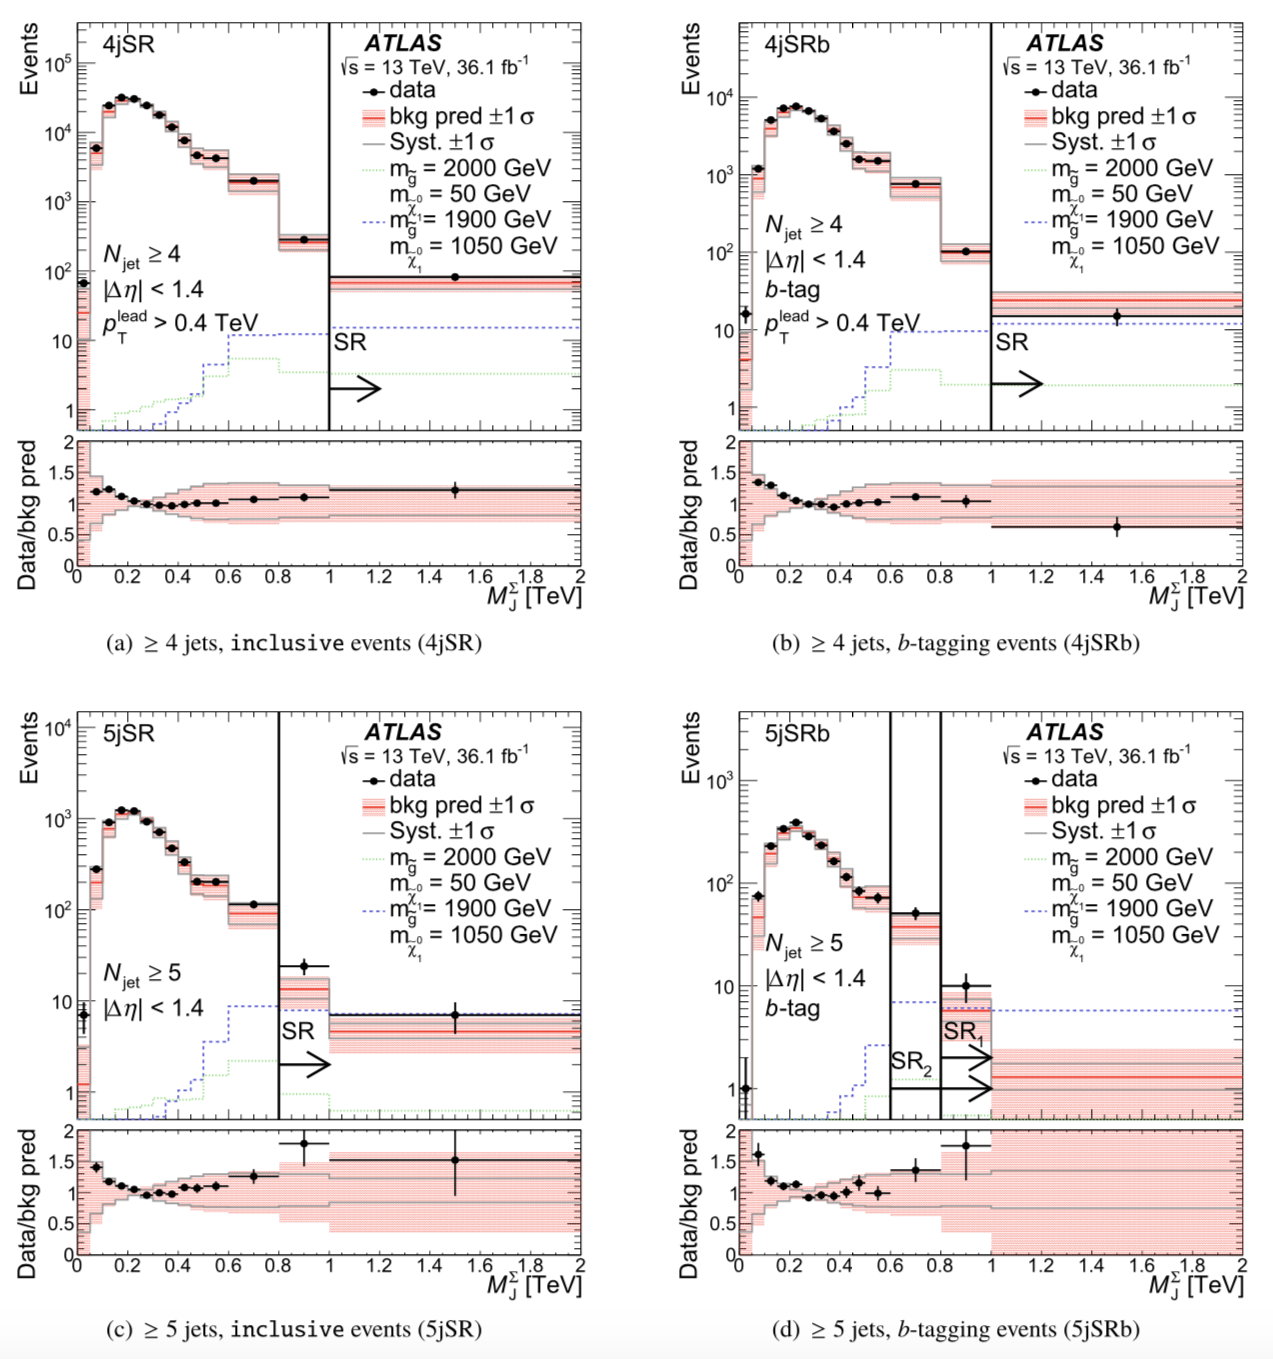
\includegraphics[width=0.8\linewidth]{results_mj_dists}
\caption{Distribution of $M_J^{\Sigma}$ in the four-jet inclusive (4jSR), four-jet b-tag (4jSRb), five-jet inclusive
(5jSR), and five-jet b-tag (5jSRb) regions.
The solid red lines show the predicted $M_J^{\Sigma}$ distributions, along with the total uncertainty shaded in red.
The black dots show the observed $M_J^{\Sigma}$ distributions.
The corresponding $M_J^{\Sigma}$ cuts are indicated with the solid black vertical line and arrow for each region.
Two separate signal regions are defined for the 5jSRb region, one with an $M_J^{\Sigma}$ cut of $0.6~TeV$,
and one with a cut of $0.8~TeV$.
The green and blue dashed lines show the predicted $M_J^{\Sigma}$ contribution from cascade-decay signal events
from two different mass points.
}
\label{fig:results_mj_dists}
\end{figure}

In the four-jet signal regions, no excess of events was observed.
In the five-jet signal regions, an excess of events were observed, but these excesses are not statistically
significant.

Predicted and observed yields in all signal regions are shown in figure\ref{fig:results_yields_table},
including the number of events in the corresponding normalization region, $N_{NR}$, and the statistical and systematic
uncertainties on the background yield predictions in those regions.

\begin{figure}[!ht]
    \centering
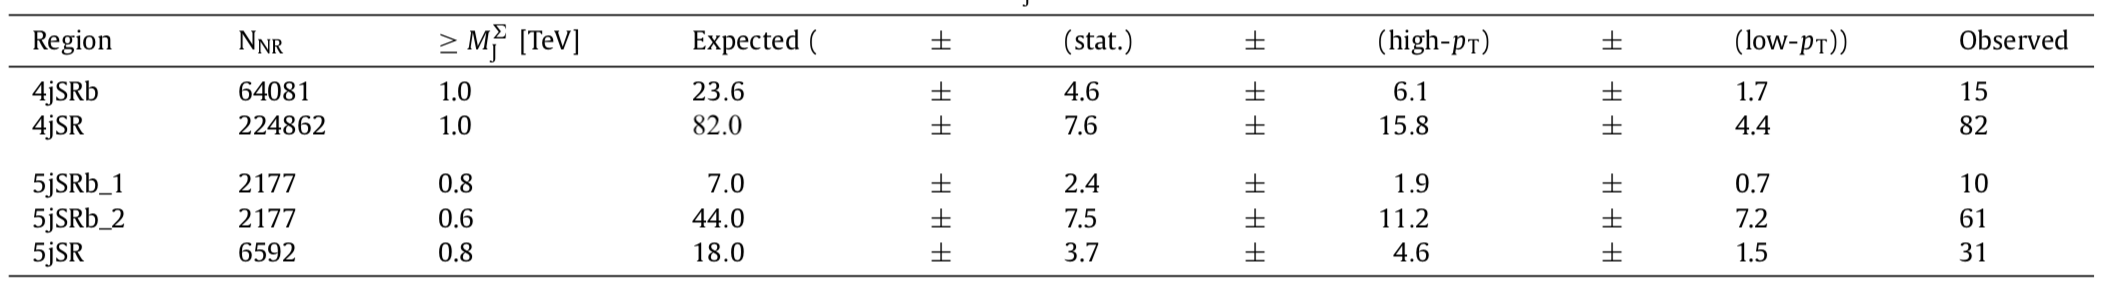
\includegraphics[width=0.8\linewidth]{results_yields_table}
\caption{Predicted and observed yields in all signal regions used in the analysis.
The number of events in the corresponding normalization regions, $N_{NR}$ is shown.
For each signal region, the minimum value of $M_J^{\Sigma}$ used to define that region is also shown.
Additionally, the statistical uncertainty on the background yield, as well as the two systematic uncertainties,
derived from the high-$p_T$ and low-$p_T$ UDRs are shown.}
\label{fig:results_yields_table}
\end{figure}

\section{Statistical Interpretation}\label{sec:results_stats}

\section{Observed and Expected Limits}\label{sec:results_limits}

\begin{figure}[!ht]
    \centering
    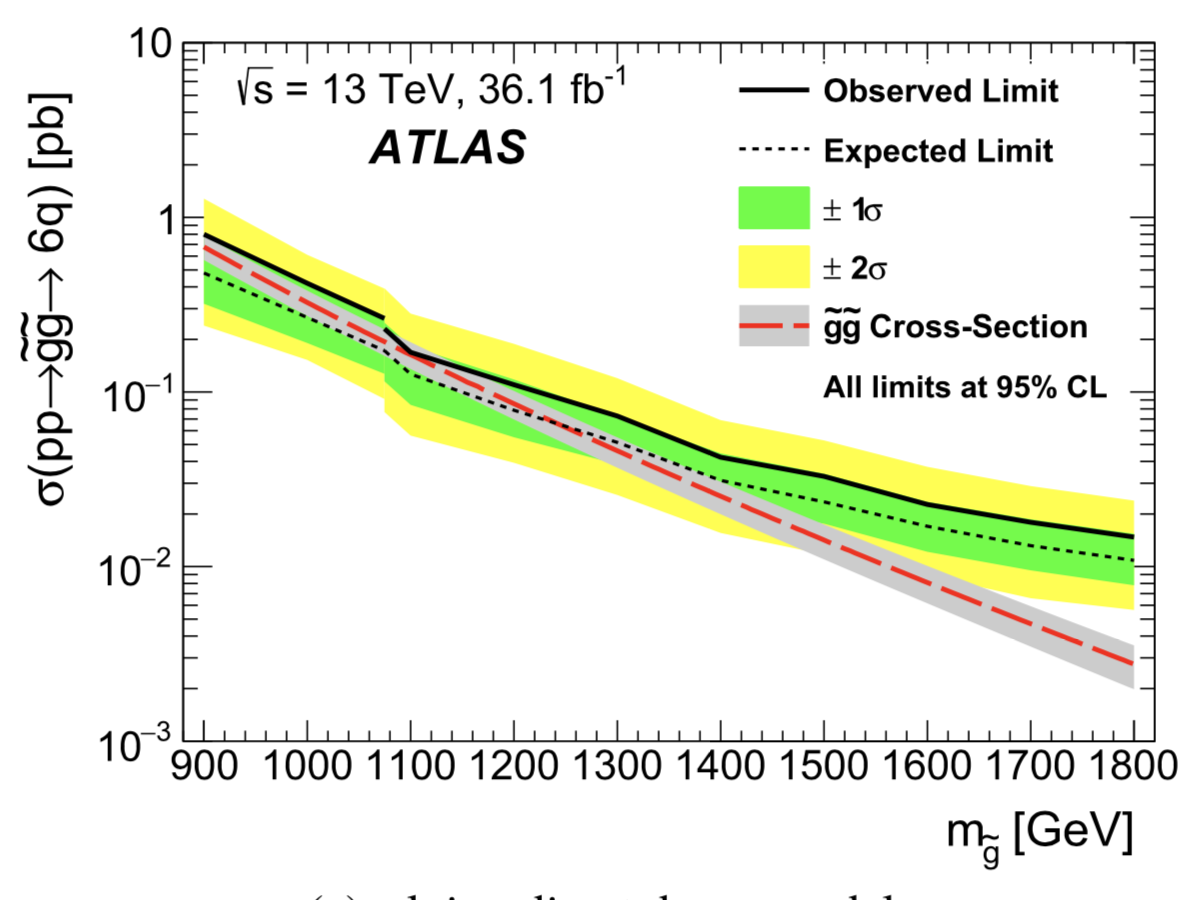
\includegraphics[width=0.8\linewidth]{results_six_quark_limits}
    \caption{Predicted and observed cross-section limits for the direct decay model over a range of $m_{\tilde{g}}$
    values.
    Also shown are the estimated gluino pair production cross-sections at each mass point.}
\label{fig:results_six_quark_limits}
\end{figure}

\begin{figure}[!ht]
    \centering
    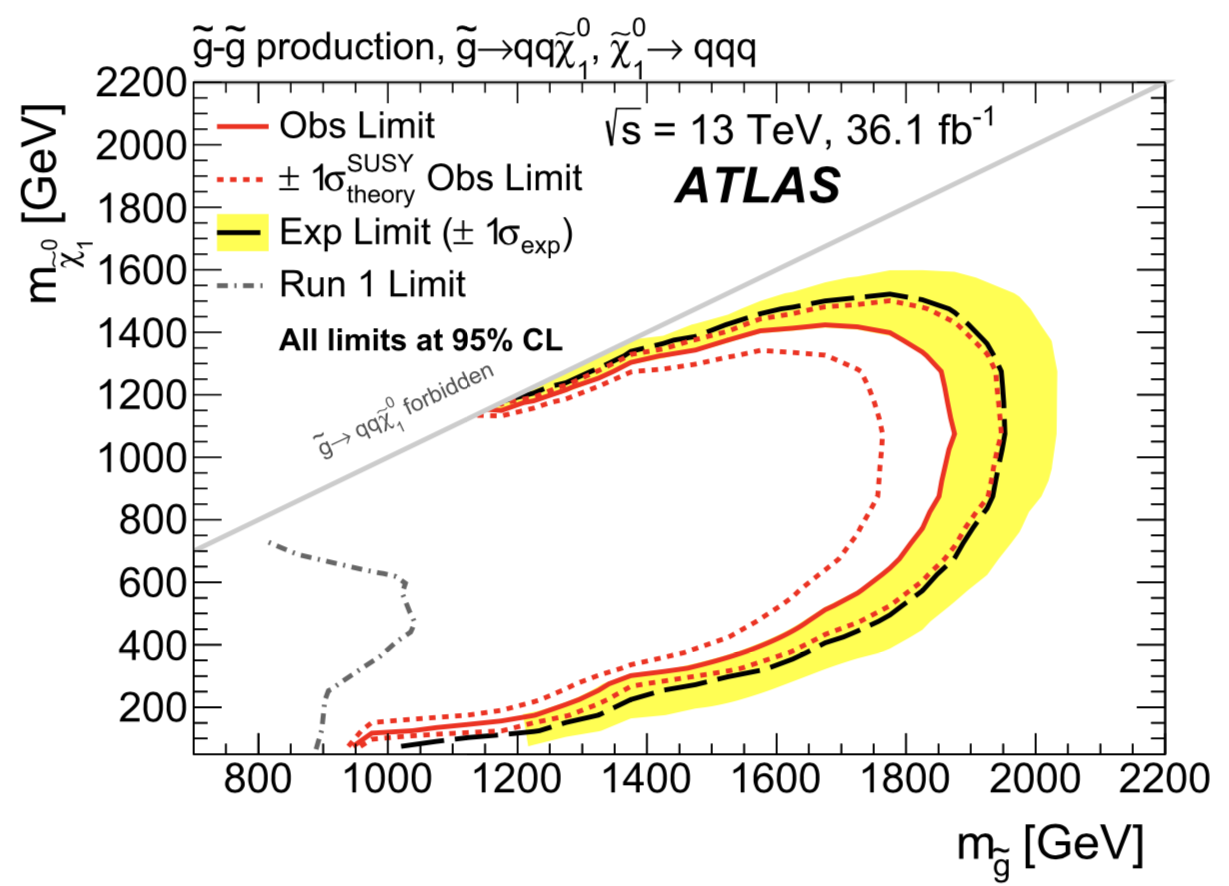
\includegraphics[width=0.8\linewidth]{results_ten_quark_limits}
    \caption{Predicted and observed limits for the cascade decay model over a range of $m_{\tilde{g}}$
and $m_{\tilde{\chi}_1^0}$ values.
    Both predicted and observed limits are shown with $1\sigma$ uncertainty bands.
    The gray dashed curve shows the limits from the Run-1 analysis.
    Due to slight excess in the signal region, the observed limit is less than expected.}
\label{fig:results_ten_quark_limits}
\end{figure}

\begin{figure}[!ht]
    \centering
    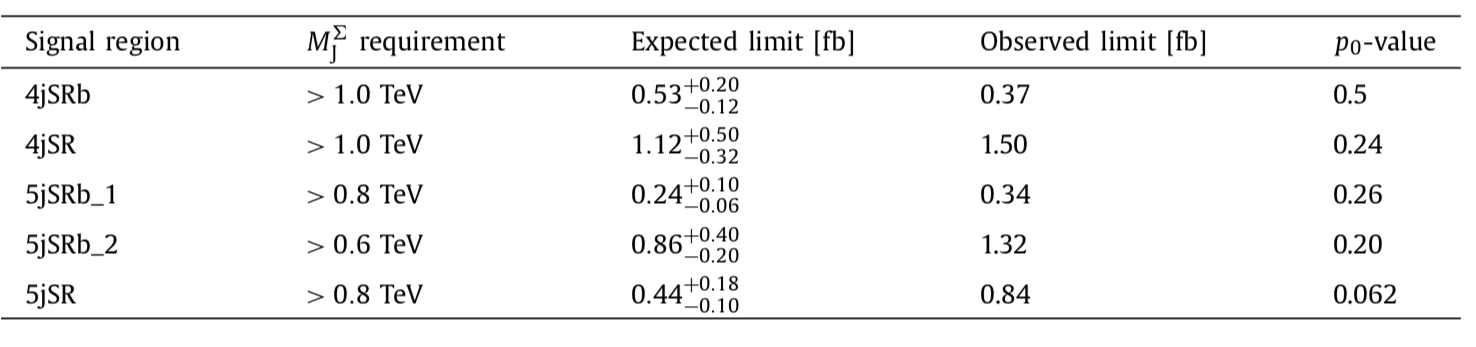
\includegraphics[width=0.8\linewidth]{results_model_ind_limits}
    \caption{}
\label{fig:results_model_ind_limits}
\end{figure}

\subsection{Ten-quark model}\label{subsec:results_limits_ten_quark}
\subsection{Six-quark model}\label{subsec:results_limits_six_quark}
\subsection{Model-independent limits}\label{subsec:results_limits_model_independent}